\subsection*{Protocolo}
Compararemos FP32 vs.\ INT8 (QSim) en validación y test. La \emph{latencia} se mide como media (y, cuando corresponda, p50/p90) sobre $N$ repeticiones en la misma máquina. Se reporta además el \emph{tamaño del modelo}. Nuestro objetivo de optimización es reducir tamaño bajo la restricción de no degradar la precisión más de $\leq 2$ puntos.

\subsection*{Ablaciones}
(i) \emph{per-tensor} vs.\ \emph{per-channel} (pesos); (ii) simétrica vs.\ asimétrica (activaciones); (iii) percentil fijo vs.\ SA (enfriamiento simulado); (iv) con/sin fusión Conv+ReLU.

\subsection*{Resultados principales}

\begin{table}[h]
\centering
\caption{Comparativa FP32 vs.\ INT8 (QSim) en MNIST.}
\begin{tabular}{lrrrr}
\toprule
Modo & Val (\%) & Test (\%) & Mean (ms) & Tamaño \\
\midrule
FP32      & 86.44 & 87.19 & 2361.2 & 80.16 KB \\
INT8-QSim & 87.06 & 87.87 & 6316.4 & 20.04 KB \\
\bottomrule
\end{tabular}
\end{table}

\subsection*{Discusión}
La PTQ con ajuste de percentiles mediante SA mantiene la precisión e incluso mejora ligeramente la generalización respecto a FP32 (en test, $\Delta=+0.68$ puntos), a la vez que reduce el tamaño $\sim 4\times$ (80.16~KB $\rightarrow$ 20.04~KB). La ganancia marginal de precisión se interpreta como un efecto de regularización por \emph{clipping} de valores extremos inducido por la cuantización.

La latencia del simulador en NumPy aumenta por (i) ausencia de kernels optimizados (convoluciones con bucles) y (ii) coste adicional de cuantizar/decuantizar y re-cuantizar. Estos tiempos son \emph{indicativos del motor funcional}, no del rendimiento en hardware con soporte INT8 o librerías BLAS, donde cabe esperar aceleración. El objetivo del trabajo —minimizar tamaño con restricción de precisión— queda satisfecho holgadamente.

% \subsection*{Matriz de confusión}
% A continuación se muestran las matrices de confusión para FP32 e INT8-QSim sobre el conjunto de test.
% \begin{figure}[h]
% \centering
% 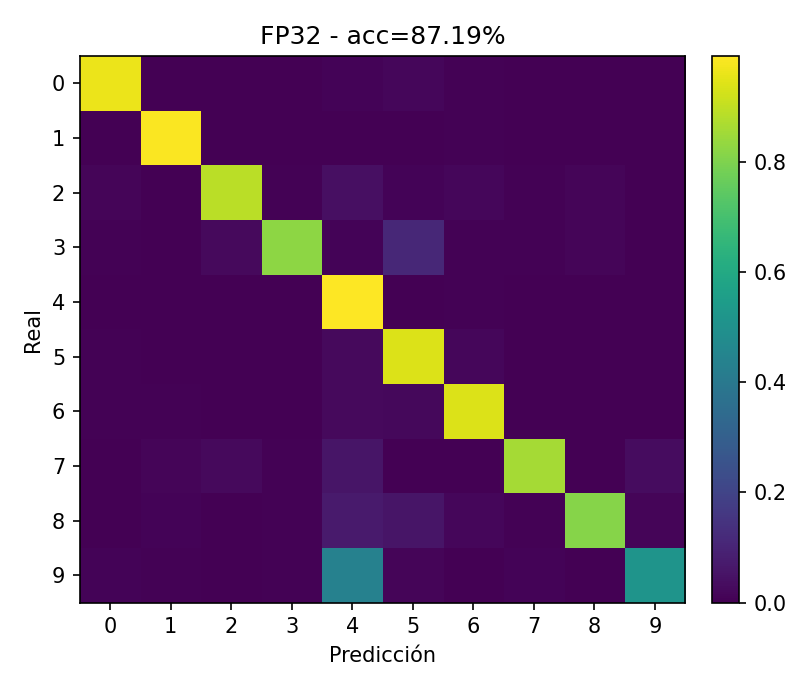
\includegraphics[width=.45\linewidth]{../results/figuras/confusion_fp32.png}\hfill
% 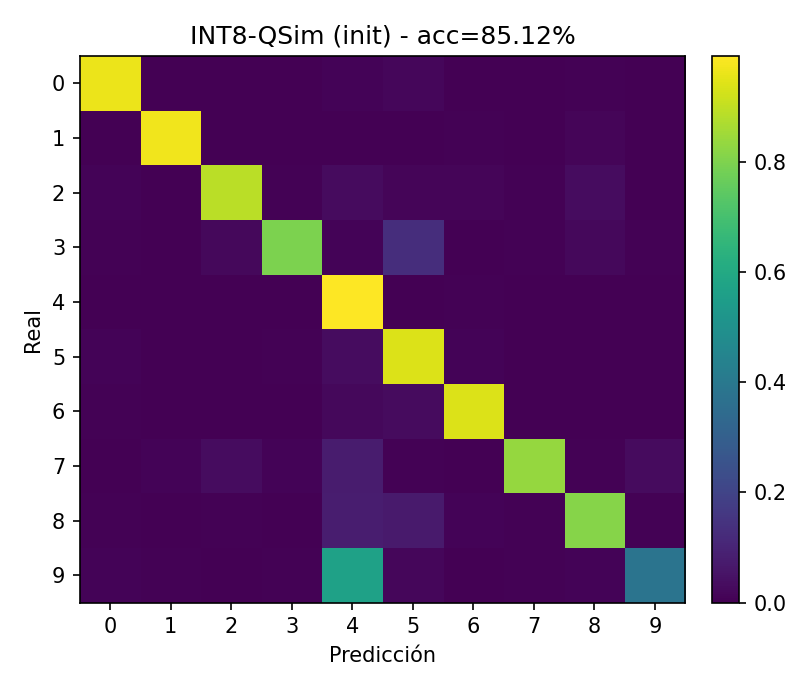
\includegraphics[width=.45\linewidth]{../results/figuras/confusion_int8.png}
% \caption{Matriz de confusión en test para FP32 (izquierda) e INT8-QSim (derecha).}
% \end{figure}

